%----------------------------------------------------------------------------------------
%	PACKAGES AND OTHER DOCUMENT CONFIGURATIONS
%----------------------------------------------------------------------------------------

\documentclass[paper=a4, fontsize=11pt]{scrartcl} % A4 paper and 11pt font size

% ---- Entrada y salida de texto -----

\usepackage[T1]{fontenc} % Use 8-bit encoding that has 256 glyphs
\usepackage[utf8]{inputenc}
%\usepackage{fourier} % Use the Adobe Utopia font for the document - comment this line to return to the LaTeX default

% ---- Idioma --------

\usepackage[spanish, es-tabla]{babel} % Selecciona el español para palabras introducidas automáticamente, p.ej. "septiembre" en la fecha y especifica que se use la palabra Tabla en vez de Cuadro

% ---- Otros paquetes ----
\usepackage{csquotes} %Para permitir el uso de comillas Quotes https://tex.stackexchange.com/questions/36812/isnt-there-any-other-way-of-doing-double-quotes-in-latex-besides
\usepackage[hyphens]{url} % ,href} %para incluir URLs e hipervínculos dentro del texto (aunque hay que instalar href)
\usepackage{hyperref}
\usepackage{color}
\usepackage{graphics,graphicx, floatrow} %para incluir imágenes y notas en las imágenes
\usepackage{graphics,graphicx, float} %para incluir imágenes y colocarlas

\graphicspath {{./img/}}

\usepackage{listings}  %para introducir comandos
\lstset{basicstyle=\ttfamily,
  showstringspaces=false,
  commentstyle=\color{red},
  keywordstyle=\color{blue}
}
% Para hacer tablas comlejas
%\usepackage{multirow}
%\usepackage{threeparttable}

%\usepackage{sectsty} % Allows customizing section commands
%\allsectionsfont{\centering \normalfont\scshape} % Make all sections centered, the default font and small caps

\usepackage{fancyhdr} % Custom headers and footers
\pagestyle{fancyplain} % Makes all pages in the document conform to the custom headers and footers
\fancyhead{} % No page header - if you want one, create it in the same way as the footers below
\fancyfoot[L]{} % Empty left footer
\fancyfoot[C]{} % Empty center footer
\fancyfoot[R]{\thepage} % Page numbering for right footer
\renewcommand{\headrulewidth}{0pt} % Remove header underlines
\renewcommand{\footrulewidth}{0pt} % Remove footer underlines
\setlength{\headheight}{13.6pt} % Customize the height of the header

\setlength\parindent{0pt} % Removes all indentation from paragraphs - comment this line for an assignment with lots of text

\newcommand{\horrule}[1]{\rule{\linewidth}{#1}} % Create horizontal rule command with 1 argument of height


%----------------------------------------------------------------------------------------
%	TÍTULO Y DATOS DEL ALUMNO
%----------------------------------------------------------------------------------------

\title{	
\normalfont \normalsize 
\textsc{\textbf{Ingeniería de Servidores (2021-2022)} \\ Grado en Ingeniería Informática \\ Universidad de Granada} \\ [25pt] % Your university, school and/or department name(s)
\horrule{0.5pt} \\[0.4cm] % Thin top horizontal rule
\huge Memoria Práctica 3 \\ % The assignment title
\horrule{2pt} \\[0.5cm] % Thick bottom horizontal rule
}

\author{Adrián Acosa Sánchez} % Nombre y apellidos

\date{\normalsize\today} % Incluye la fecha actual

%----------------------------------------------------------------------------------------
% DOCUMENTO
%----------------------------------------------------------------------------------------

\begin{document}

\maketitle % Muestra el Título

\newpage %inserta un salto de página

\tableofcontents % para generar el índice de contenidos
 
\newpage

%----------------------------------------------------------------------------------------
%	Cuestión 1
%----------------------------------------------------------------------------------------

\section{Identificación, monitorización y recuperación de RAID}

Para empezar con el ejercicio, partimos de una máquina virtual con un RAID 5 de 4 discos virtuales. Para hacer que falle, quitamos uno de los discos y añadimos otro vacío.

Para ver el estado de nuestros discos hacemos uso de la opción -D de mdadm de la siguiente manera

\begin{lstlisting}[language=bash]
	mdadm -D [nom_dispositivo]
\end{lstlisting}

En este caso tenemos en nuestra máquina virtual lo siguiente:

\begin{figure}[H]
	\centering
	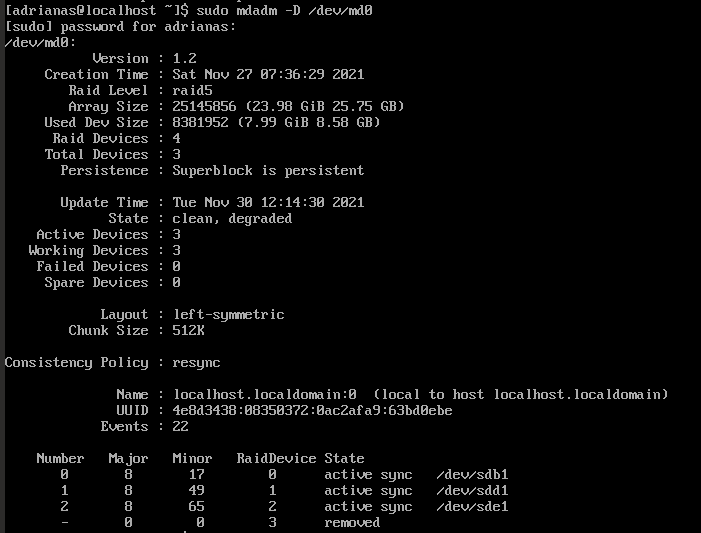
\includegraphics[scale=0.4]{graphics/img1}
	\caption{Se puede apreciar que hay un disco del RAID que aparece como eliminado, aunque el sistema sigue en funcionamiento al no suponer un error grave.}
\end{figure}

Haciendo uso del comando journalctl y buscando como palabra clave el dispositivo md0 en este caso, vemos que no supone un error grave el haber quitado uno de los discos que componían el RAID.

El comando a utilizar para ver esto es el siguiente:

\begin{lstlisting}[language=bash]
	journalctl -k -f | grep md0
\end{lstlisting}

\begin{figure}[H]
	\centering
	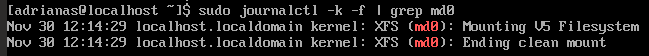
\includegraphics[scale=0.4]{graphics/img2}
	\caption{Podemos comprobar en la imagen que no supone un problema grave para el sistema.}
\end{figure}

Sea como sea, la forma de actuar ante estos casos es crear un log para poder informar al administrador del sistema y configurar un servicio de correo para que le notifique en caso de fallo de alguno de los dispositivos.

En primer lugar creamos un archivo de configuración al que le redirigimos el resultado de la monitorización del dispositivo afectado con el siguiente comando:

\begin{lstlisting}[language=bash]
	mdadm --detail --scan >> /etc/mdadm.conf
\end{lstlisting}

Tras crear este archivo, añadimos la variable MAILADDR con la dirección de correo del administrador del sistema para que le notifique en caso de fallo. Lo haríamos de la siguiente manera:

\begin{lstlisting}[language=bash]
	MAILADDR adrianacosa@correo.ugr.es
\end{lstlisting}

%------------------------------------------------

\subsection{Recuperadión del RAID}

Para la recuperación de nuestro RAID, tenemos que seguir los siguientes pasos:

\begin{enumerate}
	\item Añadimos el nuevo disco vacío al RAID
	\item Marcamos el disco como fallo
	\item Comprobamos si el disco ha sido marcado como fallo correctamente
	\item Retiramos el disco fallido
	\item Comprobamos los detalles del RAID
\end{enumerate}

Para ello ejecutamos los siguientes comandos:

\begin{lstlisting}[language=bash]
	mdadm --manage /dev/md0 --add /dev/sdi
	mdadm --manage /dev/md0 --fail /dev/sdb
	mdadm --manage /dev/md0 --remove /dev/sdb
	mdadm --detail /dev/md0
\end{lstlisting}

Después de ejecutar cada uno de los comandos, tendríamos el disco nuevo añadido a nuestro RAID de manera correcta.

%----------------------------------------------------------------------------------------
%	Cuestión 2
%----------------------------------------------------------------------------------------
\newpage
\section{Instalación y configuración de Zabbix 5.0}
\subsection{Instalación de Zabbix}

Antes de empezar a instalar Zabbix como tal, tenemos que instalar sus dependencias. Los paquetes necesarios para poder usar Zabbix son:

\begin{enumerate}
	\item MySQL / MariaDB
	\item Servidor web Apache
	\item PHP con las extensiones requeridas
\end{enumerate}

Primero tenemos que añadir los repositorios de zabbix a nuestro sistema:

\begin{figure}[H]
	\centering
	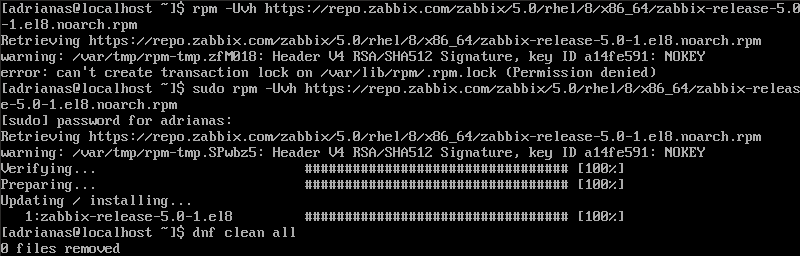
\includegraphics[scale=0.5]{graphics/img3}
	\caption{Proceso de obtención del repositorio de Zabbix}
\end{figure}

Tras esto, procedemos a intalar el servidor de Zabbix, su frontend y su agent:

\begin{lstlisting}[language=bash]
	dnf install zabbix-server-mysql
	dnf install zabbix-web-mysql
	dnf install zabbix-apache-conf
	dnf install zabbix-agent
\end{lstlisting}

El siguiente paso a realizar es crear la base de datos necesaria para nuestro servidor de Zabbix. Para ello ejecutamos los siguientes pasos dentro de mysql:

\begin{lstlisting}
	CREATE DATABASE zabbix CHARACTER SET utf8 collate utf8_bin;
	CREATE USER zabbix@localhost IDENTIFIED BY 'password';
	GRANT ALL PRIVILEGES ON zabbix.* TO zabbix@localhost;
\end{lstlisting}

\begin{figure}[H]
	\centering
	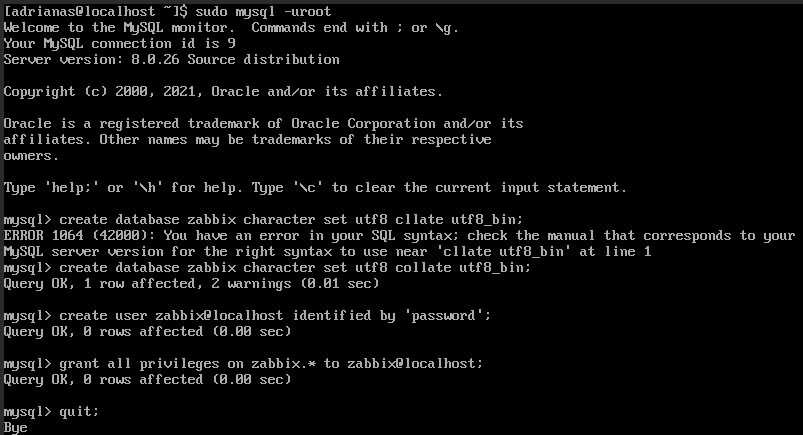
\includegraphics[scale=0.5]{graphics/img4}
	\caption{Puesta a punto de la base de datos de Zabbix}
\end{figure}
Ahora tenemos que importar los datos iniciales para el servidor. Esto se realiza con el siguiente comando:
\begin{lstlisting}[language=bash]
	zcat /usr/share/doc/zabbix-server-mysql*/create.sql.gz \
	| mysql -uzabbix -p zabbix
\end{lstlisting}

Una vez hecho esto tendremos que realizar los siguientes pasos:

\begin{enumerate}
	\item Descomentamos la linea DBPassword=password del archivo /etc/zabbix/zabbix\_server.conf.

	\item Descomentamos la linea php\_value[date.timezone] = Europe/Riga del archivo /etc/php-fpm.d/zabbix.conf .

	\item Activamos el servidor Zabbix (zabbix-server, zabbix-agent, httpd y php-fpm) con "systemctl" para que se inicie al iniciar el sistema.
	\item Configuramos el frontend de Zabbix desde la página http://127.0.0.1/zabbix
\end{enumerate}

Una cosa a tener en cuenta antes de acabar la instalación es que hay que configurar SELinux para poder iniciar los servicios de Zabbix. En concreto, hay que activar los booleanos de httpd\_can\_connnect\_zabbix y httpd\_can\_network\_connect\_db.
\\\\
Durante la puesta en marcha del servidor, he tenido algunos problemas ya que no me dejaba reiniciar los servicios necesarios para activar Zabbix. En concreto he tenido que ejecutar journalctl -xe y viendo el error he visto que era necesario ejecutar un comando:

\begin{lstlisting}[language=bash]
	semodule -X 300 -i my-zabbixserver.pp
\end{lstlisting}

Tras esto, todo ha funcionado correctamente y tendríamos toda la instalación completa.

\subsection{Configuración de Zabbix}

Ahora vamos a pasar a configurar SELinux para que permita que el backend de zabbix se pueda conectar con su frontend. Para ello ejecutamos el siguiente comando:

\begin{lstlisting}[language=bash]
	sudo setenforce 0
\end{lstlisting}

También tenemos que añadir los puertos de zabbix y de httpd al firewall para que nos permita conectarnos:

\begin{lstlisting}[language=bash]
	sudo firewall-cmd \
	--add-port={80,10051,10050}/tcp --permanent
	sudo firewall-cmd --reload
\end{lstlisting}
Una vez hecho esto, ya podremos configurar la página web que nos proporciona Zabbix. Nada más entrar en la web nos salta una página de puesta a punto para que configuremos la interfaz.

\begin{figure}[H]
	\centering
	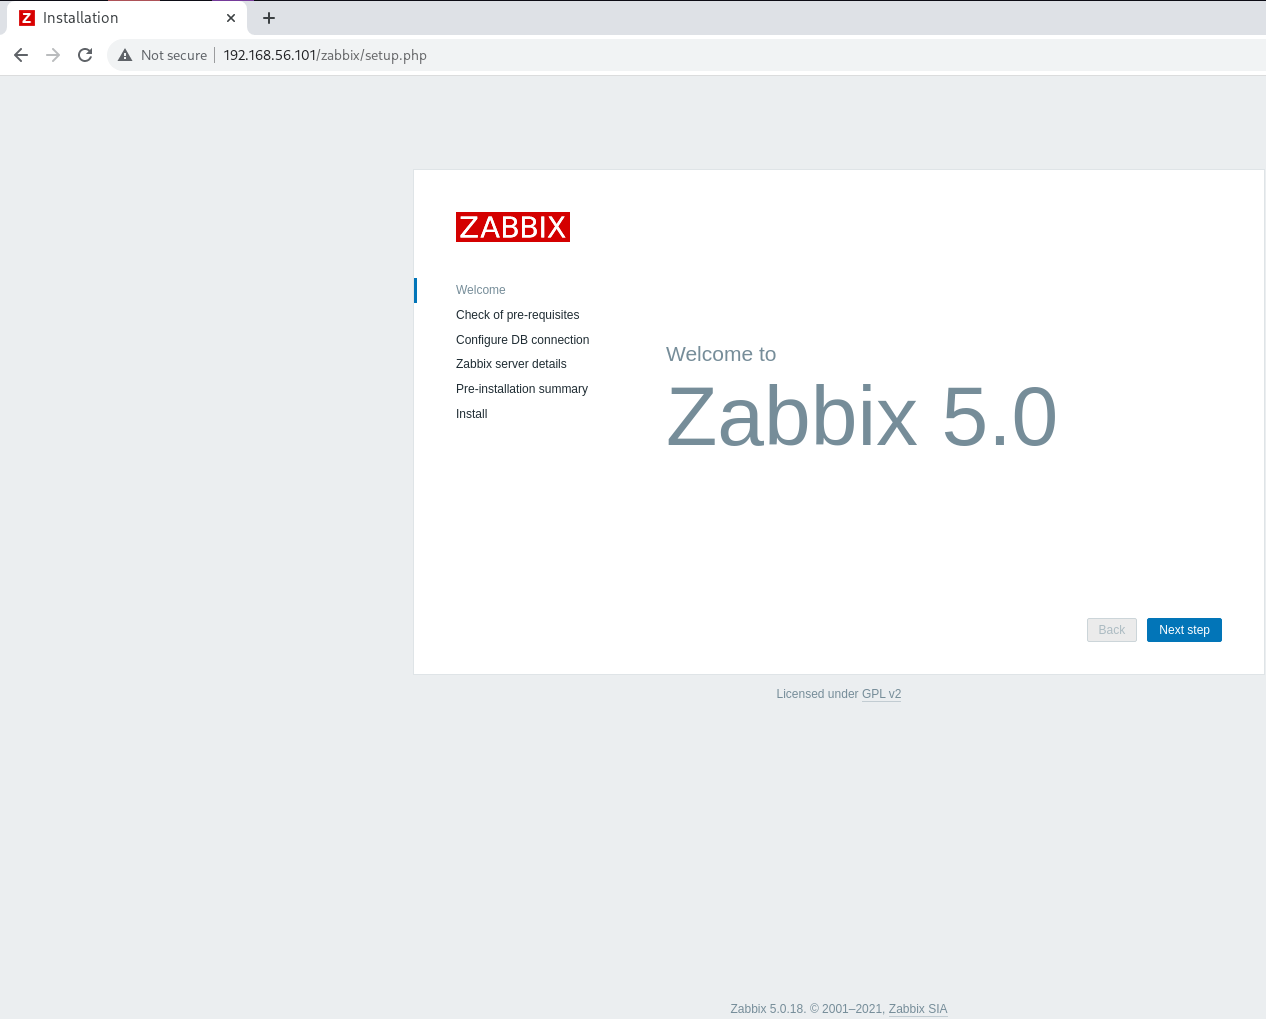
\includegraphics[scale=0.3]{graphics/img5}
	\caption{Página inicial de "setup" de Zabbix}
\end{figure}

Si le damos a "Next step"  nos lleva a la siguiente página donde podremos comprobar si tenemos todos los requisitos para poder configurar la interfaz web:

\begin{figure}[H]
	\centering
	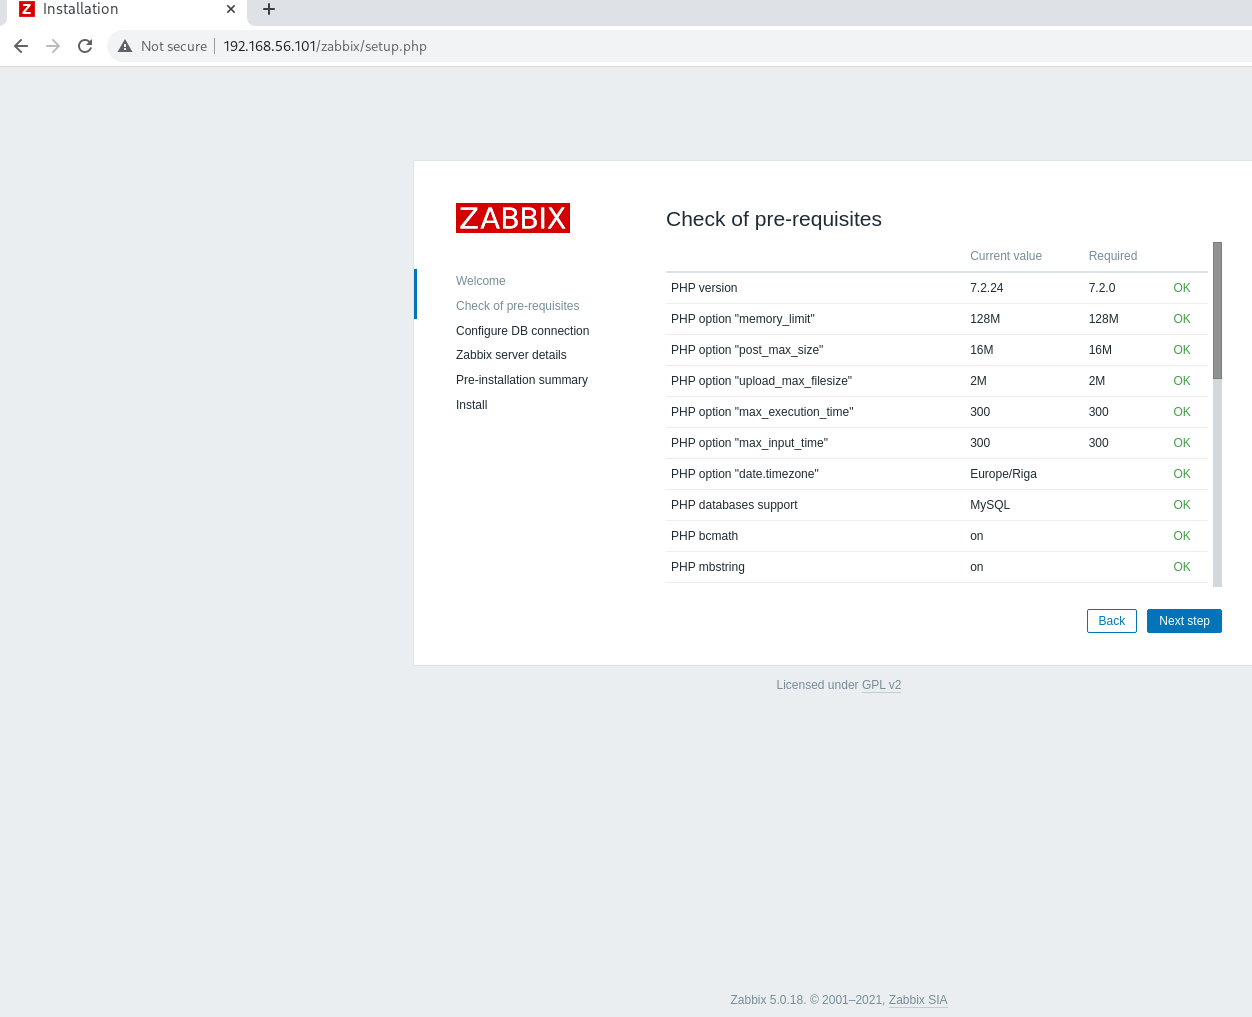
\includegraphics[scale=0.3]{graphics/img6}
	\caption{Página de comprobación de prerequisitos}
\end{figure}

Una vez hemos comprobado que todos los requisitos se cumplen, pasamos al siguiente paso que consiste en configurar la conexión a la base de datos. Para ello tenemos que recordar los datos que pusimos en la configuración de MySQL.

\begin{figure}[H]
	\centering
	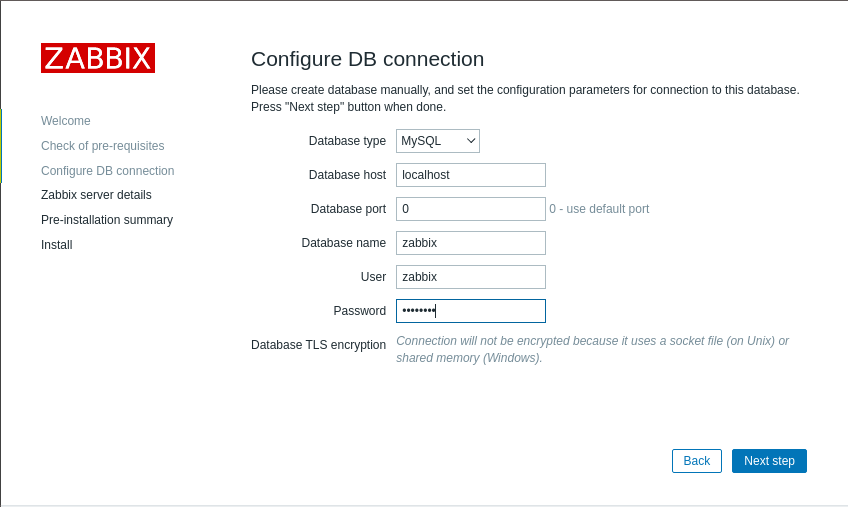
\includegraphics[scale=0.4]{graphics/img7}
	\caption{Rellenamos los datos de acuerdo a las credenciales de MySQL}
\end{figure}

En la siguiente página nos encontramos con la información relativa a donde se va a alojar el servidor y qué nombre queremos ponerle al servicio.

\begin{figure}[H]
	\centering
	
\includegraphics[scale=0.4]{graphics/img8}
	\caption{En este caso le ponemos el nombre zabbixrockylinux.com}
\end{figure}

Ahora en las dos siguientes capturas podemos ver un sumario de todos los datos que hemos introducido para poder asegurarnos de si está todo bien, y un mensaje de éxito en la configuracion.

\begin{figure}[H]
	\centering
	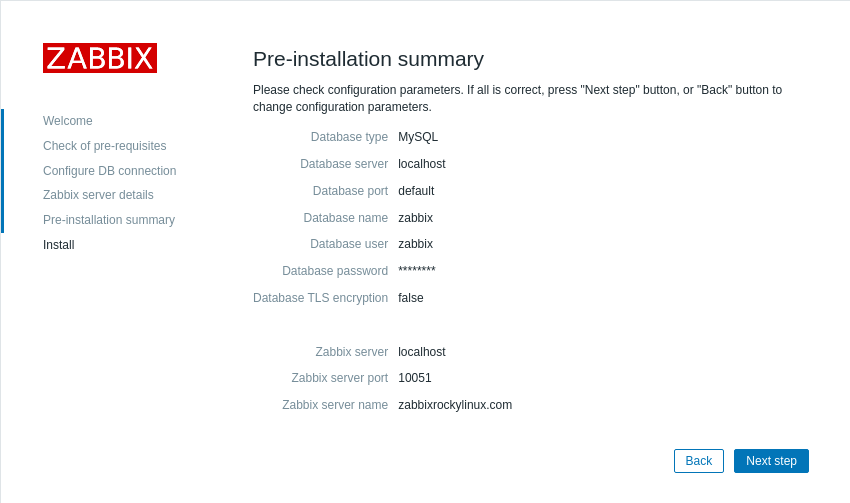
\includegraphics[scale=0.4]{graphics/img9}
	\caption{Resumen de la instalación}
\end{figure}

\begin{figure}[H]
	\centering
	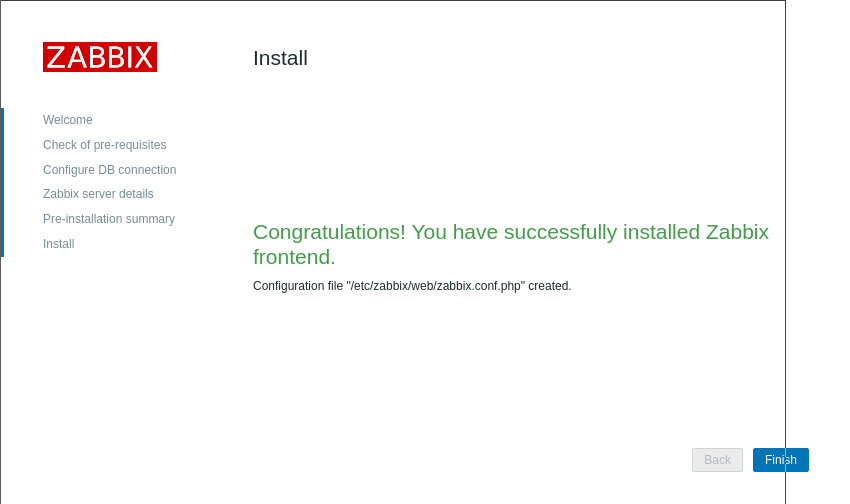
\includegraphics[scale=0.4]{graphics/img10}
	\caption{Mensaje de éxito en la instalación del frontend de zabbix}
\end{figure}

Tras esto ya tendríamos Zabbix configurado. Lo último que tenemos que hacer antes de entrar al servicio es conocer las credenciales por defecto, que en este caso son:

\begin{lstlisting}
	Username: Admin
	Password: zabbix
\end{lstlisting}

\begin{figure}[H]
	\centering
	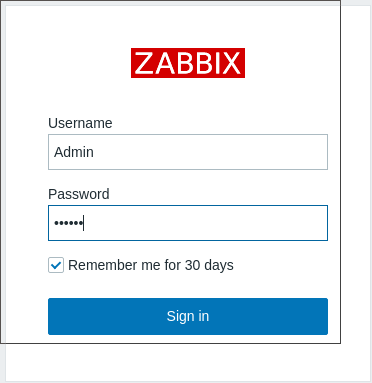
\includegraphics[scale=0.4]{graphics/img11}
	\caption{Página de inicio de sesión}
\end{figure}

\begin{figure}[H]
	\centering
	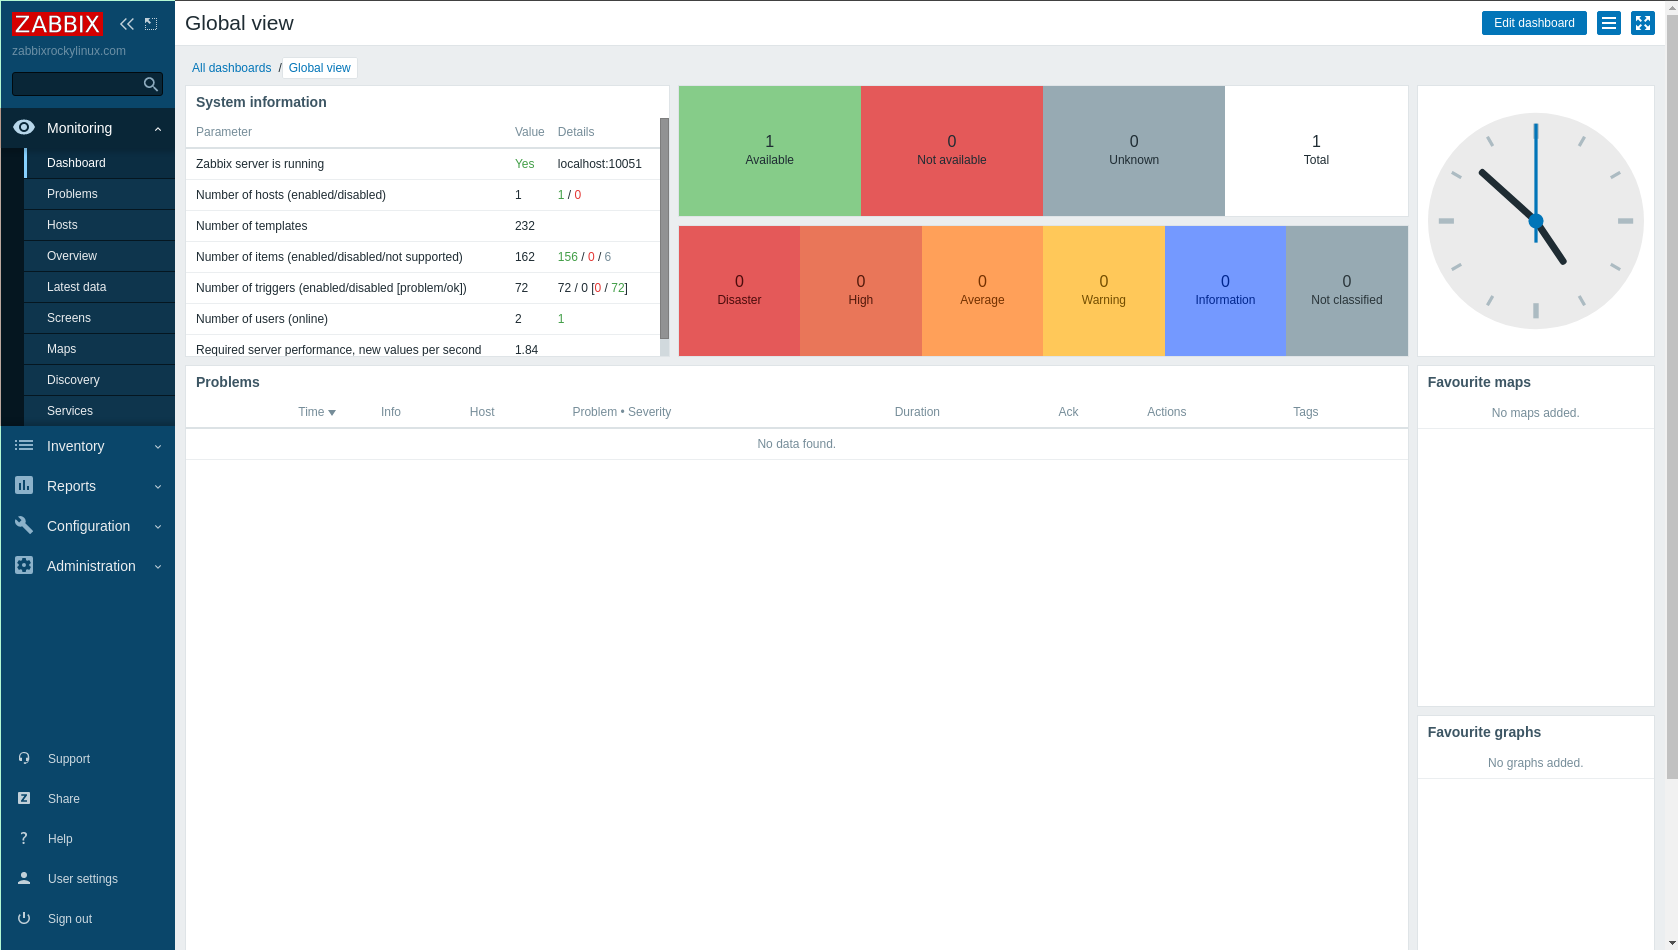
\includegraphics[scale=0.28]{graphics/img12}
	\caption{Dashboard de zabbix}
\end{figure}

\newpage
\subsection{Monitorización de HTTP y SSH con Zabbix}

Antes de empezar aclarar que las IP de ambos servidores cambian porque lo he hecho en días diferentes y con máquinas distintas.

El servidor de Zabbix está alojado en una máquina con Ubuntu Server en el que previamente hemos hecho las siguientes configuraciones:

\begin{figure}[H]
	\centering
	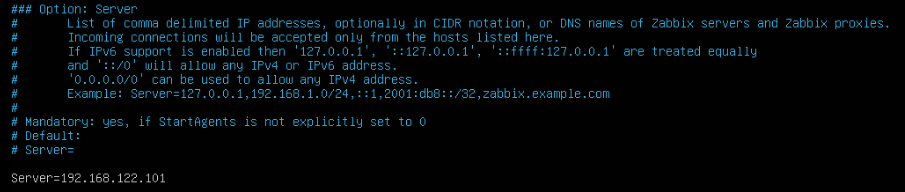
\includegraphics[scale=0.5]{graphics/img20}
	\caption{Configuración de $/etc/zabbix/zabbix\_agentd.conf$ en Ubuntu (1)}
\end{figure}

\begin{figure}[H]
	\centering
	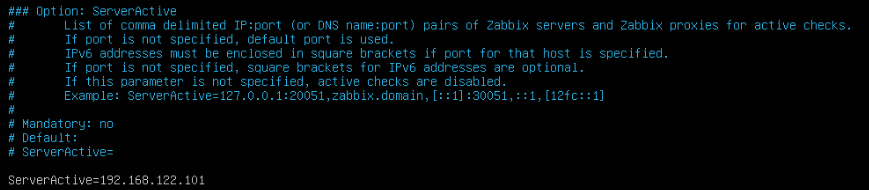
\includegraphics[scale=0.5]{graphics/img21}
	\caption{Configuración de $/etc/zabbix/zabbix\_agentd.conf$ en Ubuntu (2)}
\end{figure}

En CentOS tenemos que indicar la IP del servidor de Zabbix de la siguiente manera:

\begin{figure}[H]
	\centering
	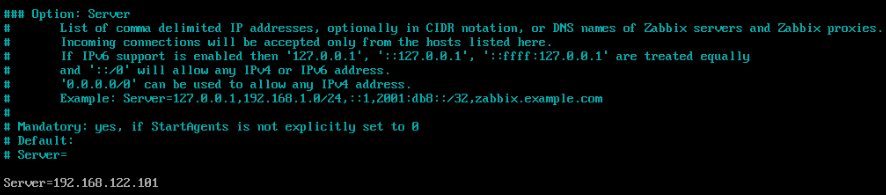
\includegraphics[scale=0.5]{graphics/img22}
	\caption{Configuración de $/etc/zabbix/zabbix\_agentd.conf$ en CentOS (1)}
\end{figure}

\begin{figure}[H]
	\centering
	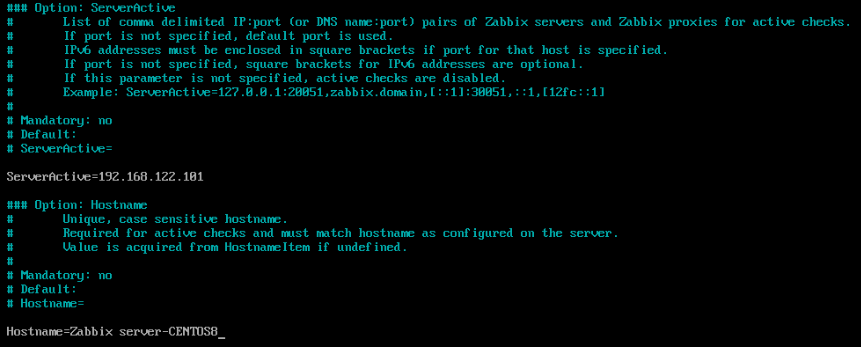
\includegraphics[scale=0.5]{graphics/img23}
	\caption{Configuración de $/etc/zabbix/zabbix\_agentd.conf$ en CentOS (2)}
\end{figure}

Una vez tenemos hecho esto, tenemos que ir al frontend de Zabbix al menú de Configuration/Hosts y le damos al botón de Create Host para crear el host de Ubuntu.

\begin{figure}[H]
	\centering
	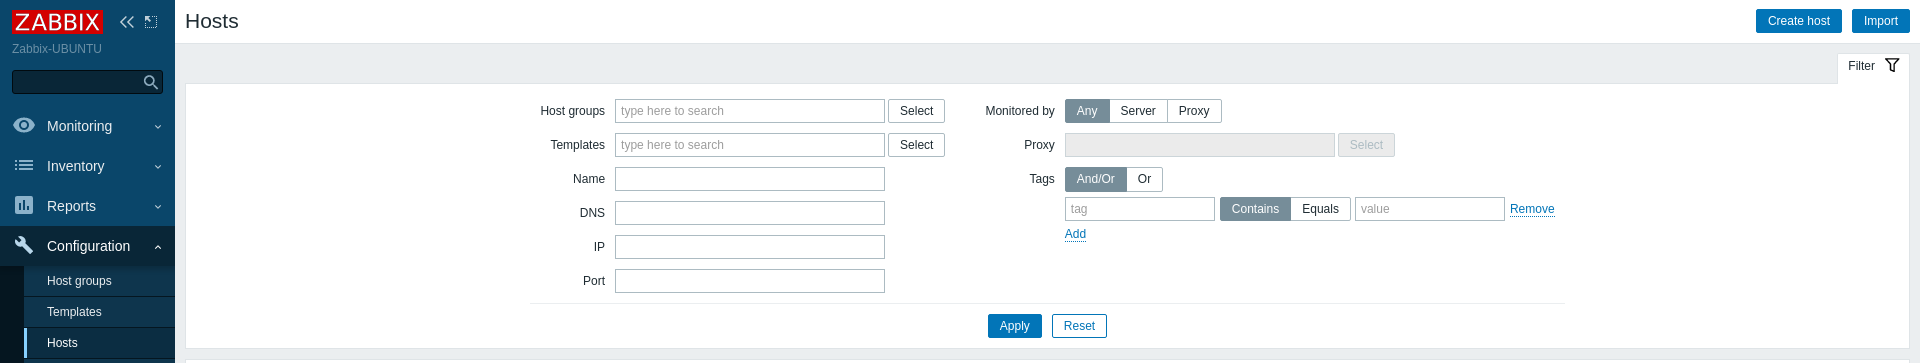
\includegraphics[scale=0.25]{graphics/img24}
	\caption{Metemos el Host en los grupos de Linux Server, Virtual Machine y Zabbix Servers. Tambien tenemos que cambiar el puerto a 10051 como indicamos en la configuracion.}
\end{figure}

\newpage
Una vez hecho esto comprobamos que se ha creado correctamente:

\begin{figure}[H]
	\centering
	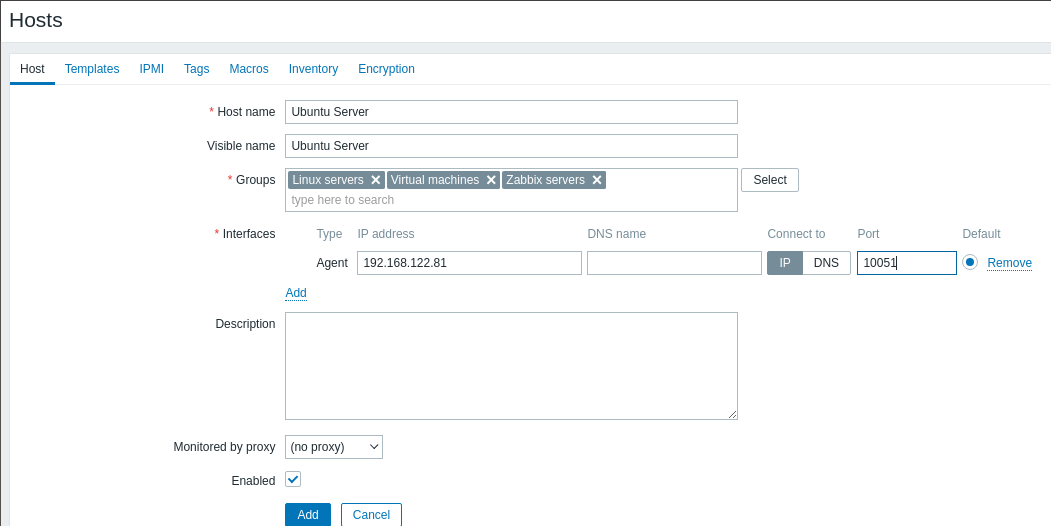
\includegraphics[scale=0.4]{graphics/img25}
	\caption{Listado de Host en el Frontend de Zabbix}
\end{figure}

Para poder realizar la monitorización de los servicios de SSH y HTTP tenemos que añadirle al Host una serie de Templates que proporciona Zabbix:

\begin{figure}[H]
	\centering
	
\includegraphics[scale=0.25]{graphics/img26}
	\caption{Listado de Templates añadidos al Host}
\end{figure}

Para poder monitorizar nuestro servidor de CentOS también tenemos que añadir un nuevo Host:

\begin{figure}[H]
	\centering
	
\includegraphics[scale=0.5]{graphics/img27}
	\caption{Creación del Host para CentOS}
\end{figure}

También es necesario añadirle los mismos templates que al Servidor principal menos el de Zabbix server para poder realizar su monitorización de los servicios SSH y HTTP.

\begin{figure}[H]
	\centering
	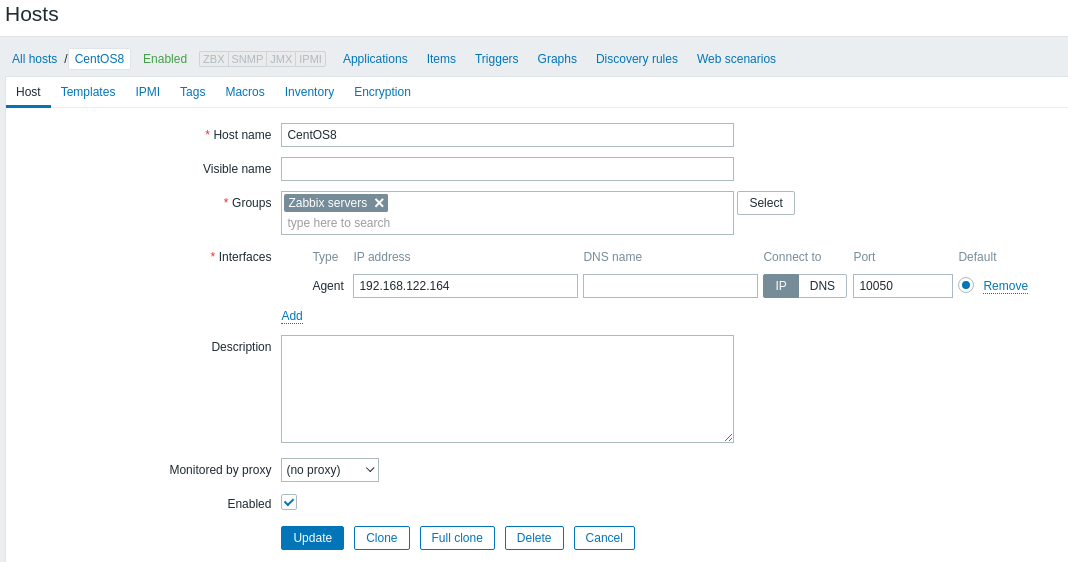
\includegraphics[scale=0.4]{graphics/img28}
	\caption{Listado de Templates para CentOS8}
\end{figure}

\newpage
Una vez hemos terminado de configurar todo lo necesario para la monitorización de dichos servicios podemos empezar a añadir unos widgets a nuestro dashboard para ayudarnos a visualizar la actividad en ambos servicios.

Para ello nos vamos al menú Monitoring/dashboard y añadimos un widget como el siguiente:

\begin{figure}[H]
	\centering
	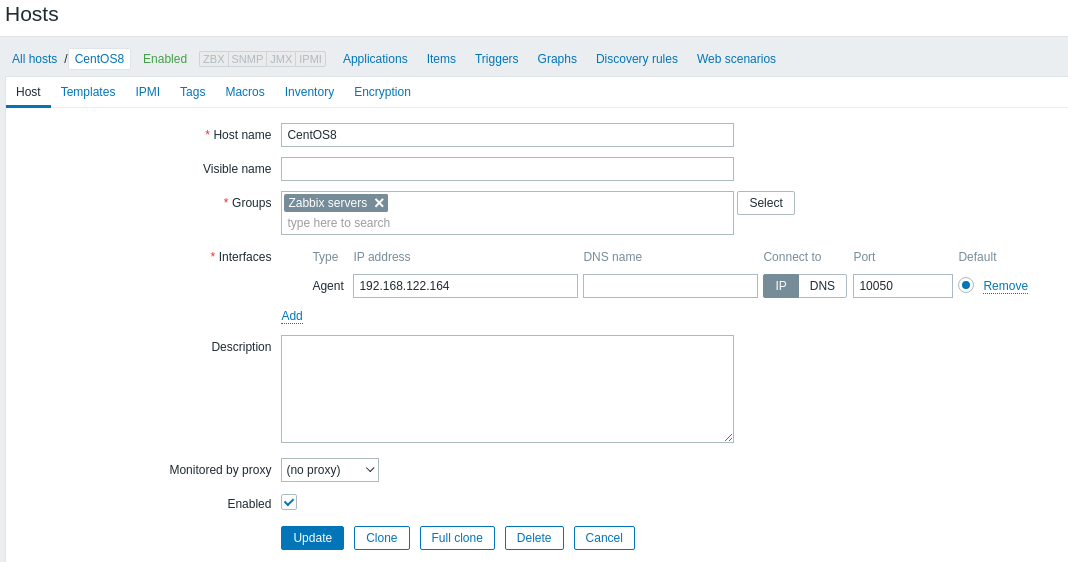
\includegraphics[scale=0.4]{graphics/img28}
	\caption{Creación de un widget de monitorización de ambos servicios}
\end{figure}


\newpage
\subsection{Monitorización de otro servidor con Zabbix}

Finalmente vamos a hacer una monitoriación del servidor de CentOS.
Para ello vamos al Host, pinchamos en items y le damos a Create Item:

\begin{figure}[H]
	\centering
	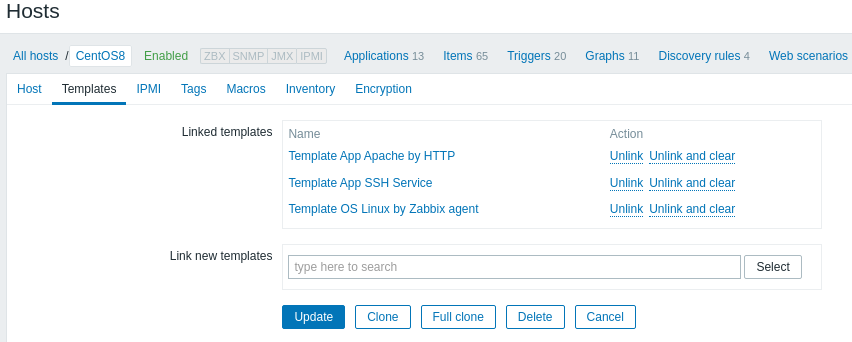
\includegraphics[scale=0.5]{graphics/img29}
	\caption{Creación del item para la monitorizacion de SSH de CentOS}
\end{figure}

Para probar si funciona vamos al final de la página a la sección de test y probamos si funciona:

\begin{figure}[H]
	\centering
	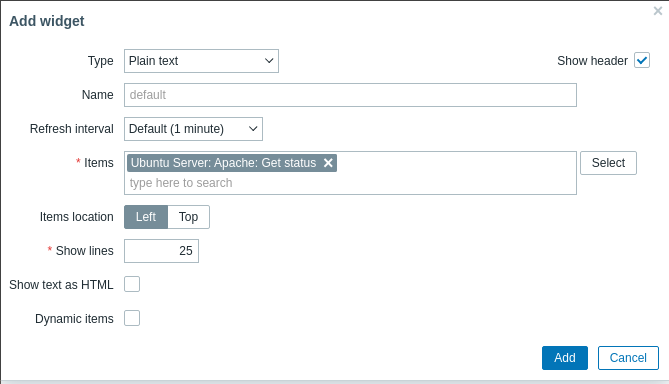
\includegraphics[scale=0.5]{graphics/img30}
	\caption{Test de la monitorizacion de SSH en CentOS}
\end{figure}

\newpage
Para HTTP es exactamente lo mismo pero en vez de poner ssh se pone http en nombre del servicio como aparece en la imagen:

\begin{figure}[H]
	\centering
	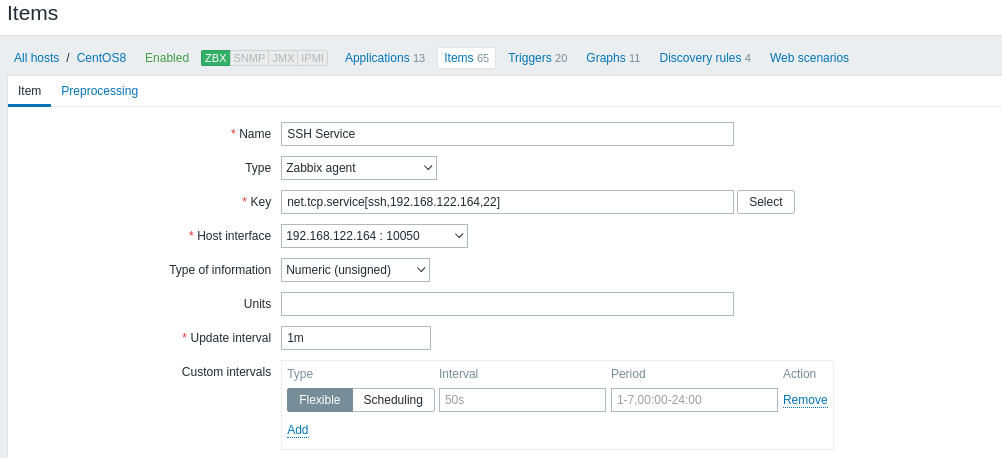
\includegraphics[scale=0.4]{graphics/img31}
	\caption{Creación de ítem de monitorización de HTTP para CentOS}
\end{figure}

%----------------------------------------------------------------------------------------
%	Cuestión 2
%----------------------------------------------------------------------------------------
\newpage
\section{Instalación y configuración de Ansible}
Ansible es un motor opensource que automatiza los procesos para preparar la infraestructura, gestionar la configuración, implementar aplicaciones y organizar los sistemas, entre otros procedimientos de TI.

Ansible permite instalar sistemas de sofware, automatizar las tareas diarias, preparar la infraestructura, mejorar la seguridad y el cumplimiento, ejecutar parches en los sistemas y compartir la automatización en toda una empresa.

\subsection{Instalación de Ansible}

Para empezar, vamos a ver como se instala ansible en nuestro sistema. Lo primero que haremos sera instalar los paquetes adicionales para linux empresarial (EPEL) a partir del siguiente comando:

\begin{lstlisting}[language=bash]
	sudo dnf install epel-release
\end{lstlisting}

\begin{figure}[H]
	\centering
	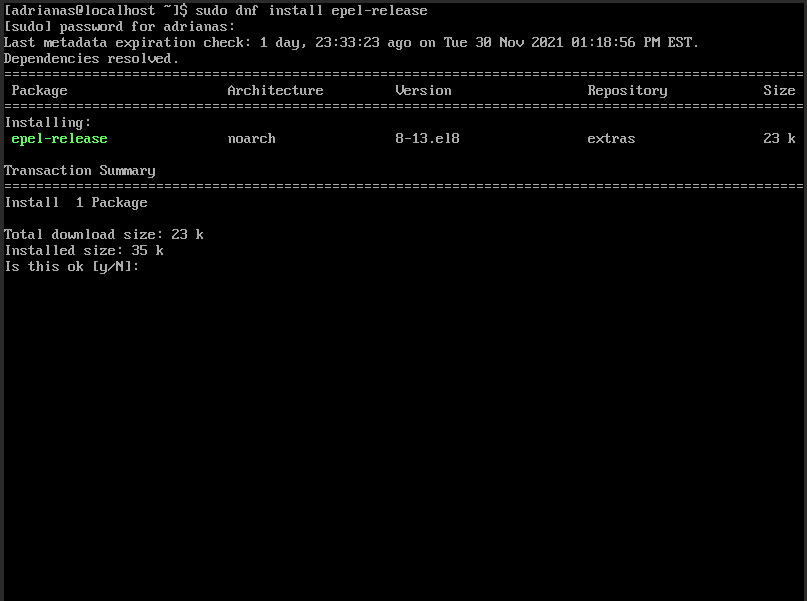
\includegraphics[scale=0.4]{graphics/img13}
	\caption{Instalación del repositorio de EPEL}
\end{figure}

\newpage
Tras esto ya tendremos acceso al paquete de ansible en nuestro sistema. Para instalarlo tenemos que ejecutar:

\begin{lstlisting}[language=bash]
	sudo dnf install ansible
\end{lstlisting}

\begin{figure}[H]
	\centering
	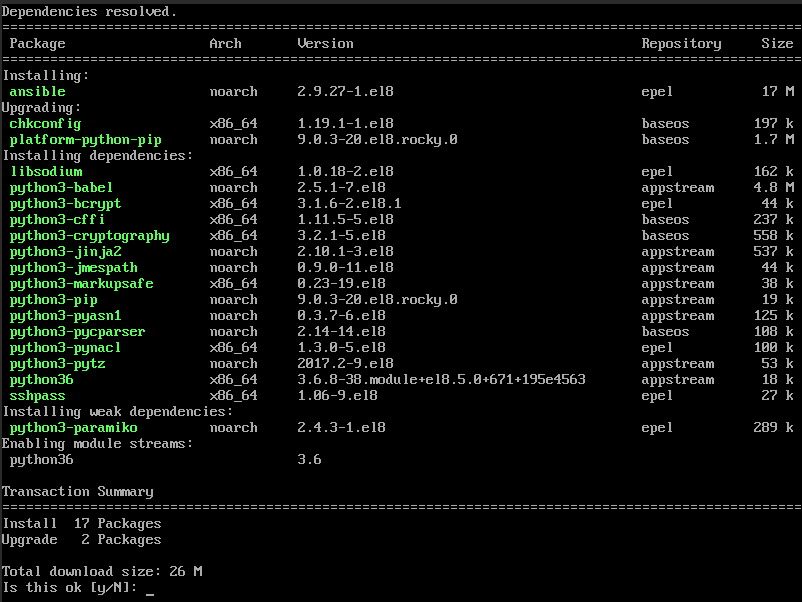
\includegraphics[scale=0.4]{graphics/img14}
	\caption{Instalación del paquete de ansible}
\end{figure}

Una vez hecho esto ya tendremos disponible ansible en nuestro sistema y podemos comprobarlo mediante la ejecución del comando:

\begin{lstlisting}[language=bash]
	ansible --version
\end{lstlisting}

\begin{figure}[H]
	\centering
	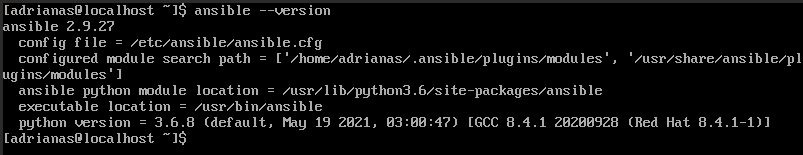
\includegraphics[scale=0.4]{graphics/img15}
	\caption{Versión de ansible para comprobar que está correctamente instalado}
\end{figure}

\newpage
\subsection{Configuración de Ansible}

Antes de configurar nada, tenemos que saber qué maquinas queremos gestionar a traves del uso de Ansible. Para ello lo primero que tenemos que conocer es la ip de cada uno ya que nos conectaremos por ssh a cada una de las máquinas.

Las máquinas de las que dispongo son 2:

\begin{enumerate}
	\item CentOS8 con IP 192.168.56.102
	\item Otra CentOS8 pero con IP 192.168.56.110
\end{enumerate}

Lo siguiente que haremos será configurar el servicio ssh, como hemos visto en la Práctica 2, en nuestra máquina con ansible y copiaremos la clave pública ssh a cada una de las dos máquinas.
\\\\
Una vez tengamos configurados los servicios ssh en cada una de las máquinas, editaremos el archivo /etc/ansible/hosts introduciendo al principio del archivo las IP de los dos servidores que queremos gestionar. Si quisiéramos gestionar servidores de apache, tendríamos que meter sus direcciones IP debajo de la etiqueta [webservers].

\begin{figure}[H]
	\centering
	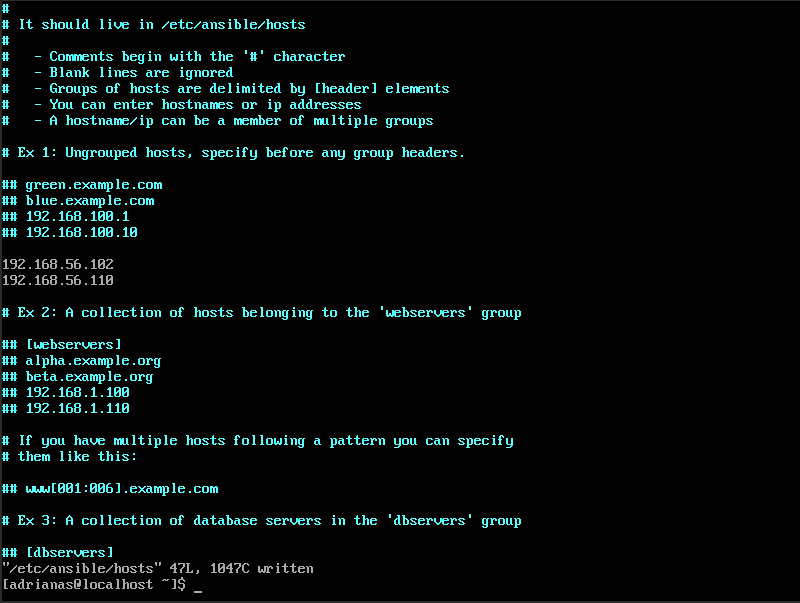
\includegraphics[scale=0.4]{graphics/img16}
	\caption{Configuración del archivo /etc/ansible/hosts. Añado las dos IP de las dos máquinas CentOS.}
\end{figure}

\newpage
Ahora que ya tenemos todas las configuraciones correctas, es hora de probar a hacer un ping mediante ansible a cada una de las máquinas o a todas a la vez con las siguientes órdenes:

\begin{lstlisting}[language=bash]
	ansible -m ping 192.168.56.102
	ansible -m ping 192.168.56.110
	ansible -m ping all
\end{lstlisting}

\begin{figure}[H]
	\centering
	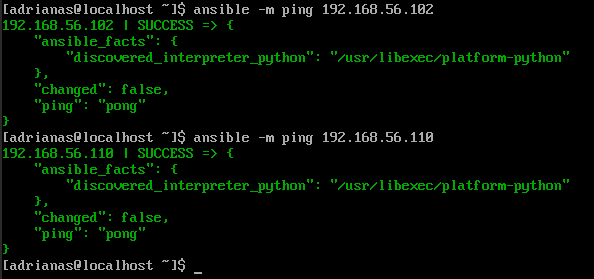
\includegraphics[scale=0.4]{graphics/img17}
	\caption{Prueba de ping a ambas máquinas CentOS}
\end{figure}

La opción -m indica el uso de un módulo específico, en este caso ping. Para poder ejecutar comandos de shell tendríamos que hacer lo mismo pero en vez de usar la orden ping, tendríamos que usar shell -a '<comando-de-shell>' como aparece en la siguiente imagen.

Antes de probar algún comando de shell, en la máquina en la que vayamos a ejecutarlo tenemos que ejecutar el siguiente comando para que no pida la contraseña de superusuario:
\\\\
echo "\$(whoami) ALL=(ALL) NOPASSWD:ALL" | sudo tee /etc/sudoers.d/\$(whoami)
\\\\
A continuación muestro un ejemplo de la orden:

\begin{lstlisting}
	ansible -b --become-method=sudo \
	-m shell -a 'dnf update' 192.168.56.102
\end{lstlisting}

\begin{figure}[H]
	\centering
	
\includegraphics[scale=0.4]{graphics/img18}
	\caption{Prueba de ejecución de un comando shell}
\end{figure}

\newpage
Para comprobar que realmente funciona:

\begin{figure}[H]
	\centering
	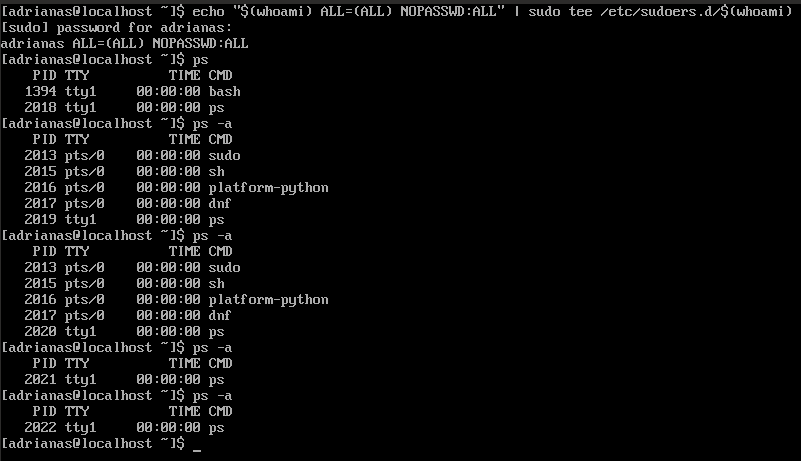
\includegraphics[scale=0.5]{graphics/img19.png}
	\caption{Se puede observar que se esta ejecutando dnf y las dependencias de ansible de forma remota, hasta que hacemos control+c.}
\end{figure}



%-------Bibliografia-----------------------------

\newpage
\section{Bibliografía}

\footnote{Instalación y configuración de Zabbix server en Rocky Linux 8 o CentOS8}
\textcolor{blue}{\url{https://techviewleo.com/install-and-configure-zabbix-server-on-rocky-linux/}}

\footnote{Instalación de Zabbix server en Rocky Linux 8 o CentOS8}
\textcolor{blue}{\url{https://www.zabbix.com/download?zabbix=5.0\&os_distribution=centos&os_version=8\&db=mysql\&ws=apache}}

\footnote{Gestión de RAID y reparación de fallos}
\textcolor{blue}{\url{https://access.redhat.com/documentation/en-\%20us/red\_hat\_enterprise\_linux/8/html/managing\_storage\_devices/managing-raid\_managing-storage-devices}}

\footnote{Instalación de Ansible en Rocky Linux 8}
\textcolor{blue}{\url{https://www.how2shout.com/linux/how-to-install-ansible-on-rocky-linux-8-or-almalinux/}}

\footnote{Conceptos básicos de Ansible}
\textcolor{blue}{\url{https://www.redhat.com/es/topics/automation/learning-ansible-tutorial}}

\footnote{Instalación de EPEL en CentOS8 o Rocky Linux 8}
\textcolor{blue}{\url{https://fedoraproject.org/wiki/EPEL/es}}

\footnote{Página del manual de linux sobre Ansible}
\textcolor{blue}{\url{https://linux.die.net/man/1/ansible}}



\end{document}
